\documentclass[titlepage]{article}
\usepackage[left=15mm,right=15mm,top=1in,bottom=1in]{geometry}
\usepackage{graphicx}

\title{Stone Identification App \\
  Software Requirements Specification}
\author{Genevieve Okon (okong), Sydney Lieng(liengsn),\\
  Niko Savas(savasn), Nick Lago(lagond),\\
  Eric Le Fort(leforte)}
\date{\today}

\begin{document}
\maketitle
\newpage

\subsection{Use Case Diagram}

  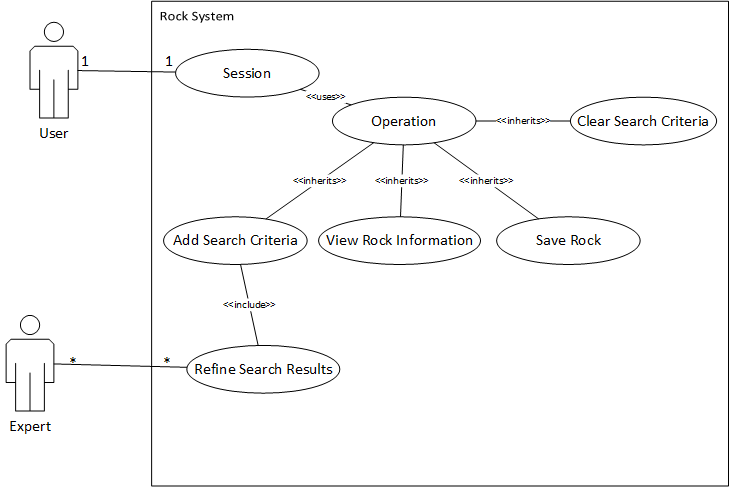
\includegraphics[scale = 0.65]{../resources/UseCaseDiagram.png}
  \subsubsection{Session}
    When the user opens the app, a session is started. During the session, the user can manage their search criteria to identify a rock, with information such as colour, size, and texture. The session is terminated when the user closes the app or is finished with their search.
  \subsubsection{Operation}
    The operation is an abstract use case. It is extended by clear search criteria, add search criteria, view rock information,view collection, and save rock.
  \subsubsection{Add Search Criteria}
    The user can add information about the rock to the search criteria to refine the list of possible matches. The information pulled from the expert's search result refinement helps to refine possible matches.
  \subsubsection{Refine Search Results}
    This use case is implemented by all experts contributing to the application. Given a set of inputs, an expert can refine a set of search results to only include those that match the inputs.
  \subsubsection{View Rock Information}
    The user can view detailed information about any given rock included in the list of matches or their collection. The information displayed is sourced from the data store of the application.
  \subsubsection{View Collection}
    The user can view their collection of saved rocks. This provides a shortlist of rocks that have been added using the "Save Rock" operation. 
  \subsubsection{Save Rock}
    The user can, at any time, add a rock to their collection.
\end{document}